% ============================================================
\chapter{Introduction \`a l'apprentissage automatique}
\label{ch:introduction}
\index{apprentissage automatique}
% ============================================================

\section{Qu'est-ce que l'apprentissage automatique~?}

\begin{definition}[Apprentissage automatique]
L'\textbf{apprentissage automatique} (\emph{machine learning}) est l'\'etude
d'algorithmes qui am\'eliorent automatiquement leurs performances sur une
t\^ache donn\'ee \`a travers l'exp\'erience (donn\'ees), sans \^etre
explicitement programm\'es pour cette t\^ache~\cite{murphy2022}.
\end{definition}

Plus formellement, suivant Tom Mitchell~: un programme apprend d'une
exp\'erience $E$ par rapport \`a une classe de t\^aches $T$ et une mesure
de performance $P$, si sa performance sur $T$, mesur\'ee par $P$, s'am\'eliore
avec l'exp\'erience $E$.

\section{Types d'apprentissage}
\label{sec:types}
\index{apprentissage!types}

\begin{center}
\begin{tikzpicture}[
  cat/.style={rectangle, draw, rounded corners, minimum width=3cm,
    minimum height=1cm, align=center, font=\small\bfseries},
  sub/.style={rectangle, draw, rounded corners, fill=white,
    minimum width=2.8cm, font=\scriptsize, align=center}
]
  \node[cat, fill=blue!15] (sup) {Supervis\'e};
  \node[cat, fill=green!15, right=2.5cm of sup] (unsup) {Non supervis\'e};
  \node[cat, fill=orange!15, right=2.5cm of unsup] (rl) {Par renforcement};

  \node[sub, below=0.4cm of sup] (s1) {R\'egression\\Classification};
  \node[sub, below=0.4cm of unsup] (s2) {Clustering\\R\'eduction dim.};
  \node[sub, below=0.4cm of rl] (s3) {Exploration\\Exploitation};

  \draw[-{Stealth}] (sup) -- (s1);
  \draw[-{Stealth}] (unsup) -- (s2);
  \draw[-{Stealth}] (rl) -- (s3);
\end{tikzpicture}
\end{center}

\subsection{Apprentissage supervis\'e}
\index{apprentissage!supervis\'e}

On dispose d'un jeu de donn\'ees $\mathcal{D} = \{(\bm{x}_i, y_i)\}_{i=1}^n$
o\`u $\bm{x}_i \in \R^d$ est un vecteur de \emph{features} (caract\'eristiques)
et $y_i$ est l'\'etiquette (\emph{label}). L'objectif est d'apprendre une
fonction $f : \R^d \to \mathcal{Y}$ telle que $f(\bm{x}) \approx y$ pour
de nouvelles donn\'ees.

\begin{itemize}
  \item \textbf{R\'egression}~: $\mathcal{Y} = \R$ (prix d'un appartement,
    temp\'erature).
  \item \textbf{Classification}~: $\mathcal{Y} = \{1, \ldots, K\}$ (spam/non-spam,
    chiffres manuscrits).
\end{itemize}

\subsection{Apprentissage non supervis\'e}
\index{apprentissage!non supervis\'e}

On dispose uniquement de $\mathcal{D} = \{\bm{x}_i\}_{i=1}^n$ sans \'etiquettes.
L'objectif est de d\'ecouvrir une structure cach\'ee~: clusters, vari\'et\'es
de faible dimension, distributions.

\subsection{Apprentissage par renforcement}
\index{apprentissage!par renforcement}

Un agent interagit avec un environnement, re\c{c}oit des r\'ecompenses, et
apprend une politique maximisant la r\'ecompense cumul\'ee. Ce paradigme
n'est pas couvert dans ce cours.

\section{Formalisation math\'ematique}
\label{sec:formalization}

\subsection{Espace des hypoth\`eses}

\begin{definition}[Espace des hypoth\`eses]
L'\textbf{espace des hypoth\`eses}\index{espace des hypoth\`eses}
$\mathcal{H}$ est l'ensemble des fonctions $h : \R^d \to \mathcal{Y}$ parmi
lesquelles l'algorithme d'apprentissage cherche la meilleure.
\end{definition}

\begin{exemple}[R\'egression lin\'eaire]
$\mathcal{H} = \{h_{\bm{w}} : \bm{x} \mapsto \bm{w}^\top \bm{x} + b
\mid \bm{w} \in \R^d, b \in \R\}$.
\end{exemple}

\subsection{Fonction de perte et risque}
\index{fonction de perte}

\begin{definition}[Fonction de perte]
Une \textbf{fonction de perte} $\ell : \mathcal{Y} \times \mathcal{Y} \to \R_+$
mesure l'erreur entre la pr\'ediction $\hat{y} = h(\bm{x})$ et la vraie
valeur $y$. Exemples courants~:
\begin{align}
  \text{Erreur quadratique~:} \quad & \ell(y, \hat{y}) = (y - \hat{y})^2 \\
  \text{Erreur 0-1~:} \quad & \ell(y, \hat{y}) = \ind[y \neq \hat{y}] \\
  \text{Log-loss~:} \quad & \ell(y, \hat{y}) = -y\log\hat{y} - (1-y)\log(1-\hat{y})
\end{align}
\end{definition}

\begin{definition}[Risque]
Le \textbf{risque} (ou erreur de g\'en\'eralisation)\index{risque} d'une
hypoth\`ese $h$ est~:
\begin{equation}
  R(h) = \E_{(\bm{x}, y) \sim P}[\ell(y, h(\bm{x}))]
\end{equation}
o\`u $P$ est la distribution jointe (inconnue) des donn\'ees.
\end{definition}

\begin{definition}[Risque empirique]
Le \textbf{risque empirique}\index{risque!empirique} est l'approximation du
risque sur les donn\'ees d'entra\^inement~:
\begin{equation}
  \hat{R}_n(h) = \frac{1}{n} \sum_{i=1}^n \ell(y_i, h(\bm{x}_i))
\end{equation}
\end{definition}

\begin{formules}[title=\textbf{Principe de minimisation du risque empirique (ERM)}]
L'algorithme d'apprentissage cherche~:
\begin{equation}
  h^* = \argmin_{h \in \mathcal{H}} \hat{R}_n(h) = \argmin_{h \in \mathcal{H}}
  \frac{1}{n} \sum_{i=1}^n \ell(y_i, h(\bm{x}_i))
  \label{eq:erm}
\end{equation}
\end{formules}

\section{Le compromis biais-variance}
\label{sec:bias-variance}
\index{biais-variance}

\begin{theoreme}[D\'ecomposition biais-variance]
Pour la perte quadratique, le risque se d\'ecompose en~:
\begin{equation}
  \E[(y - \hat{f}(\bm{x}))^2] = \underbrace{\Bias^2[\hat{f}(\bm{x})]}_{\text{biais}^2}
  + \underbrace{\Var[\hat{f}(\bm{x})]}_{\text{variance}}
  + \underbrace{\sigma^2_\varepsilon}_{\text{bruit irr\'eductible}}
\end{equation}
o\`u $\Bias[\hat{f}(\bm{x})] = \E[\hat{f}(\bm{x})] - f(\bm{x})$ et
$\sigma^2_\varepsilon = \Var[\varepsilon]$.
\end{theoreme}

\begin{center}
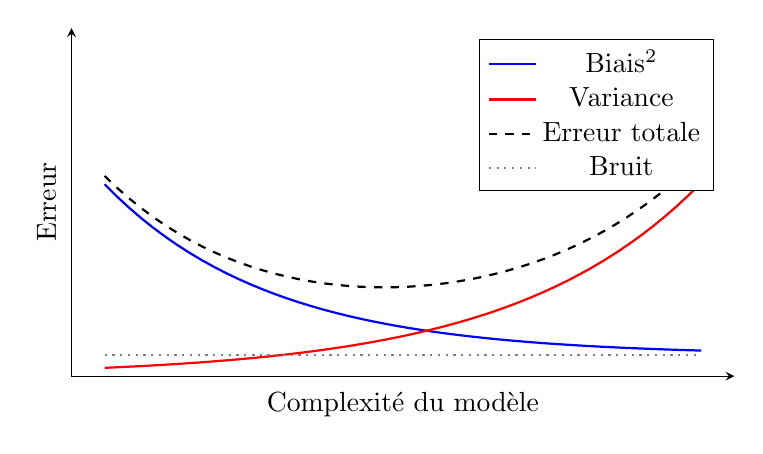
\begin{tikzpicture}
  \begin{axis}[
    width=10cm, height=6cm,
    xlabel={Complexit\'e du mod\`ele},
    ylabel={Erreur},
    xmin=0, xmax=10, ymin=0, ymax=5,
    legend pos=north east,
    axis lines=left,
    xtick=\empty, ytick=\empty
  ]
    \addplot[thick, blue, domain=0.5:9.5, samples=50] {3*exp(-0.4*x) + 0.3};
    \addlegendentry{Biais$^2$}
    \addplot[thick, red, domain=0.5:9.5, samples=50] {0.1*exp(0.35*x)};
    \addlegendentry{Variance}
    \addplot[thick, black, dashed, domain=0.5:9.5, samples=50]
      {3*exp(-0.4*x) + 0.1*exp(0.35*x) + 0.3};
    \addlegendentry{Erreur totale}
    \addplot[thick, gray, dotted, domain=0.5:9.5] {0.3};
    \addlegendentry{Bruit}
  \end{axis}
\end{tikzpicture}
\end{center}

\begin{intuition}[title=\textbf{Interpr\'etation}]
\begin{itemize}
  \item Un mod\`ele trop simple (biais \'elev\'e) ne capture pas la
    structure des donn\'ees~: \textbf{sous-apprentissage} (\emph{underfitting}).
  \item Un mod\`ele trop complexe (variance \'elev\'ee) s'adapte au bruit~:
    \textbf{surapprentissage} (\emph{overfitting}).
  \item L'objectif est de trouver le compromis optimal.
\end{itemize}
\end{intuition}

\section{\'Evaluation des mod\`eles}
\label{sec:evaluation}
\index{\'evaluation}

\subsection{D\'ecoupage des donn\'ees}

\begin{bonnepratique}[title=\textbf{Train / Validation / Test}]
\begin{itemize}
  \item \textbf{Entra\^inement} (60--80\,\%)~: pour ajuster les param\`etres.
  \item \textbf{Validation} (10--20\,\%)~: pour choisir les hyperparam\`etres.
  \item \textbf{Test} (10--20\,\%)~: pour estimer la performance finale.
    \textbf{Jamais} utilis\'e pour le choix du mod\`ele.
\end{itemize}
\end{bonnepratique}

\subsection{Validation crois\'ee}
\index{validation crois\'ee}

\begin{definition}[Validation crois\'ee $k$-fold]
On partitionne les donn\'ees en $k$ sous-ensembles (\emph{folds}).
Pour chaque fold $i$~:
\begin{enumerate}
  \item Entra\^iner sur les $k-1$ autres folds.
  \item \'Evaluer sur le fold $i$.
\end{enumerate}
L'erreur de validation crois\'ee est la moyenne des $k$ erreurs~:
\begin{equation}
  \text{CV}(k) = \frac{1}{k} \sum_{i=1}^k \hat{R}^{(i)}
\end{equation}
\end{definition}

\subsection{M\'etriques}

\begin{formules}[title=\textbf{M\'etriques courantes}]
\textbf{R\'egression~:}
\begin{align}
  \text{MSE} &= \frac{1}{n}\sum_{i=1}^n (y_i - \hat{y}_i)^2, \quad
  \text{RMSE} = \sqrt{\text{MSE}}, \quad
  R^2 = 1 - \frac{\sum(y_i-\hat{y}_i)^2}{\sum(y_i - \bar{y})^2}
\end{align}

\textbf{Classification~:}
\begin{align}
  \text{Pr\'ecision} &= \frac{VP}{VP + FP}, \quad
  \text{Rappel} = \frac{VP}{VP + FN}, \quad
  F_1 = 2 \cdot \frac{\text{Pr\'ec.} \times \text{Rappel}}{\text{Pr\'ec.} + \text{Rappel}}
\end{align}
\end{formules}

\section{Impl\'ementation~: premier mod\`ele avec scikit-learn}
\label{sec:first-model}

\begin{codeblock}[title=\textbf{Classification Iris avec scikit-learn}]
\begin{minted}{python}
import numpy as np
from sklearn.datasets import load_iris
from sklearn.model_selection import train_test_split, cross_val_score
from sklearn.neighbors import KNeighborsClassifier
from sklearn.metrics import classification_report

# Charger les donnees
X, y = load_iris(return_X_y=True)

# Decoupage train/test
X_train, X_test, y_train, y_test = train_test_split(
    X, y, test_size=0.2, random_state=42, stratify=y
)

# Modele k-NN
model = KNeighborsClassifier(n_neighbors=5)
model.fit(X_train, y_train)

# Evaluation
print(f"Accuracy test: {model.score(X_test, y_test):.4f}")
print(classification_report(y_test, model.predict(X_test)))

# Validation croisee 5-fold
scores = cross_val_score(model, X, y, cv=5, scoring="accuracy")
print(f"CV accuracy: {scores.mean():.4f} +/- {scores.std():.4f}")
\end{minted}
\end{codeblock}

\begin{codeoutput}
\begin{verbatim}
Accuracy test: 1.0000
              precision    recall  f1-score   support
           0       1.00      1.00      1.00        10
           1       1.00      1.00      1.00        10
           2       1.00      1.00      1.00        10
    accuracy                           1.00        30
CV accuracy: 0.9667 +/- 0.0211
\end{verbatim}
\end{codeoutput}

\section{Exercices}
\label{sec:exercises-ch1}

\begin{exercice}[Risque empirique]
Soit $\mathcal{D} = \{(1, 2), (2, 3.5), (3, 6)\}$ et $h_w(x) = wx$.
\begin{enumerate}
  \item Calculer $\hat{R}_3(h_w)$ avec la perte quadratique pour $w = 1.5$
    et $w = 2$.
  \item Trouver $w^*$ minimisant $\hat{R}_3(h_w)$ analytiquement.
  \item Tracer $\hat{R}_3(h_w)$ en fonction de $w$.
\end{enumerate}
\end{exercice}

\begin{exercice}[D\'ecomposition biais-variance]
\begin{enumerate}
  \item Montrer que $\E[(y - \hat{f})^2] = \Bias^2 + \Var + \sigma^2$ en
    d\'etaillant chaque \'etape.
  \item G\'en\'erer $n = 50$ points avec $y = \sin(x) + \varepsilon$,
    $\varepsilon \sim \mathcal{N}(0, 0.3)$. Ajuster des polyn\^omes de
    degr\'es 1, 3, 5, 10, 15 et illustrer le compromis biais-variance.
\end{enumerate}
\end{exercice}

\begin{exercice}[Validation crois\'ee]
\begin{enumerate}
  \item Impl\'ementer la validation crois\'ee $k$-fold \`a partir de z\'ero
    (sans \pkg{sklearn.model\_selection}).
  \item Comparer les r\'esultats de votre impl\'ementation avec
    \cli{cross\_val\_score} pour k-NN sur le dataset Iris.
  \item \'Etudier l'effet de $k$ (nombre de voisins) sur l'accuracy CV.
    Tracer la courbe accuracy vs $k$ pour $k \in \{1, 3, 5, 7, \ldots, 25\}$.
\end{enumerate}
\end{exercice}
